\documentclass[11pt,a4paper]{article}
\usepackage[english]{babel}
\renewcommand{\thesubsection}{\thesection.\alph{subsection}}

\selectlanguage{english}
\NeedsTeXFormat{LaTeX2e}
\renewcommand{\baselinestretch}{1.3}
\usepackage[utf8]{inputenc}
\usepackage{enumerate}
\usepackage{csquotes}
\usepackage{listings}
\usepackage{amsmath}
\usepackage{amsfonts}
\usepackage{amssymb}
\usepackage{afterpage}
\usepackage{lscape}
\usepackage{caption}
\usepackage{appendix}
\usepackage{enumitem}
\usepackage{upquote}
\usepackage{xcolor}
\usepackage{graphicx}
\usepackage{fancyhdr}
\usepackage{makecell}
\usepackage{mdwlist}
%Mida de marges i columnes______
\usepackage{vmargin}
\usepackage{graphicx}
\graphicspath{ {imatges/} }
\setpapersize{A4}
\setmargins{2.5cm}{1.5cm}{16.5cm} {23.42cm}{32.54pt}{1cm}{0pt}{1.5cm} 
\usepackage{multicol}
\usepackage{multirow}
\usepackage{float}
\usepackage{cancel}
\usepackage{gensymb}
\setlength{\columnsep}{1cm}
%_______________________________
%Bibliografia
\bibliographystyle{apalike}
\renewcommand{\baselinestretch}{1.2}
\usepackage[urldate=long]{biblatex}
\bibliography{refs.bib}
\usepackage{url}
%_______________________________

%Capçalera_______________________
\pagestyle{fancy}
\fancyhead[L]{Potential Aerodynamics}
\fancyhead[R]{Aerodinàmica, Mecànica de Vol i Orbital
%\includegraphics[scale=0.2]{imatges/upc.png}}
}
\setlength{\headheight}{40pt} 
%________________________________

\usepackage[hidelinks]{hyperref}
\usepackage[all]{hypcap}

\newenvironment{imatge}
{\par\medskip\noindent\minipage{\linewidth}}
{\endminipage\par\medskip}

\lstset{language=Matlab,breaklines=true}


%Taules
\usepackage{tabularx}
\usepackage{longtable}
%\usepackage[table]{xcolor}
%\usepackage[table,xcdraw]{xcolor}
%\documentclass[xcolor=table]{beamer}
\usepackage{diagbox}

%Símbol €
\usepackage[utf8]{inputenc}
\usepackage{eurosym}


%Requadrar text
\usepackage{amsthm}
\usepackage{verbatim}

%Matlab
%\usepackage{listings}
\usepackage{matlab-prettifier}

%Annex
\usepackage{appendix}

%Totes les seccions del document_________________________
\begin{document}
\begin{titlepage}


\centering
{\bfseries\LARGE Universitat Politècnica de Catalunya\par}
%\vspace{1.5cm}
{\scshape\Large Escola Superior d'Enginyeries Industrial, Aeroespacial i Audiovisual de Terrassa\par}
\vspace{2.5cm}
{\scshape\Huge Aerodynamics Project:  \\The constant strength vortex method and Prandtl's lifting line model
 \par}
\vspace{2cm}
{\itshape\Large Aerodinàmica, Mecànica de Vol i Orbital \\ 2024-25 Q2 \par}
\vspace{0.5cm}
{02/06/2025 \par}
\vspace{0.5cm}
{\scshape\Large Group 12  \par}
\vspace{0.2cm}

{\Large Lluís Ceinos, Marc \par}
{\Large Gutiérrez Portillo, Guillem \par}
{\Large Poposki Stanojkovska, Vedran \par}
\vspace{2.5cm}
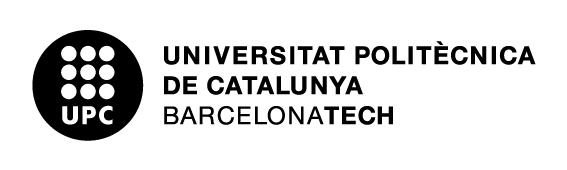
\includegraphics[width=0.4\textwidth]{imatges/logo upc negre sobre blanc.png}


\end{titlepage}
\newpage

% Índex___________________________
    \addtocontents{toc}{\hfill \textbf{Page} \par}
    \tableofcontents
    \newpage
    %\listoffigures
    %\newpage
    %\listoftables
    %\newpage
%_________________________________
\section{Introduction to the Problem}

The objective of this project is to study the flow around the surfaces of a glider airplane composed by a wing, a canard and a vertical tail plane, all attached thanks to a thin, negligible, rigid rod, as shown in Figure \ref{fig:GliderConfig}. Both wing and canard have zero sweep angle and a trapezoidal shape, with their geometries defined by the following values:

\[b = 24 m;     cr = 1.8 m;     ct = 1.2 m\]
\[b_h = 6 m;     cr_h = 1 m;     ct_h = 0.6 m\]

The airfoils employed are the NACA 22112 and NACA 0012 for the wing and canard respectively. Incidence angles are $0^\circ$ for the wing and $3^\circ$ for the canard.

\begin{figure}[H]
    \centering
    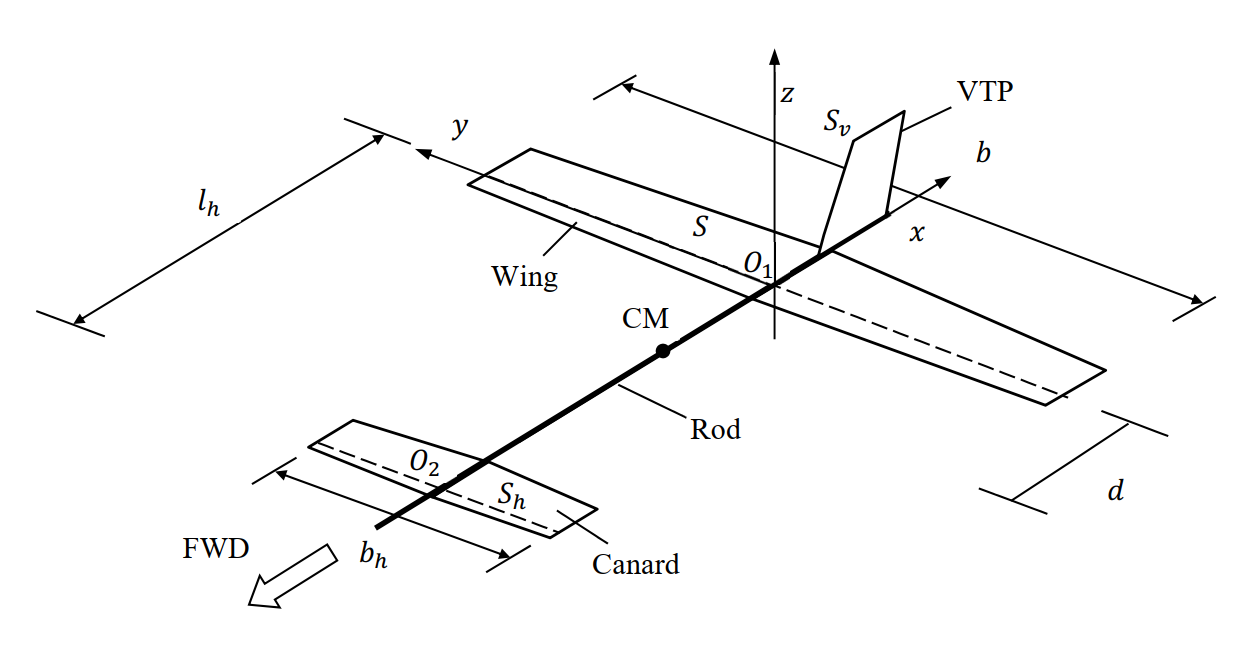
\includegraphics[width=0.8\linewidth]{imatges/gliderconfig.png}
    \caption{Configuration of the studied glider aircraft.}
    \label{fig:GliderConfig}
\end{figure}

The problem is divided into the following parts:
\begin{itemize}
    \item \textbf{Part 1:} Implementation of the constant strength vortex method. This part is itself divided in two, firstly the wing is studied with the objective to compute relevant aerodynamic coefficients, then the flow around the canard is calculated, considering it a combination of two airfoils, in order to understand the aerodynamic effects of having two areodynamic components very close together as can be observed in Figure \ref{fig:CanardConfig}.
    
    \begin{figure}[H]
        \centering
        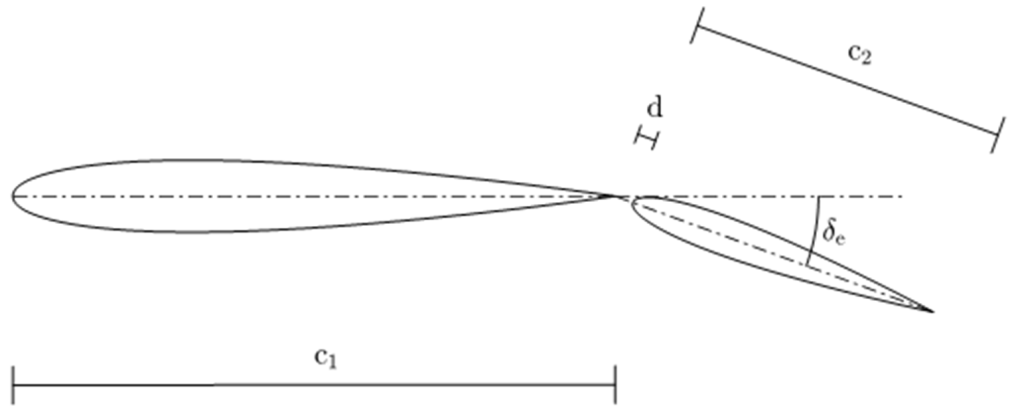
\includegraphics[width=0.4\linewidth]{imatges/canardconfig.png}
        \caption{Configuration of the canard, with two NACA 0012 in succession.}
        \label{fig:CanardConfig}
    \end{figure}
    
    \item \textbf{Part 2:} Implementation of Prandtl's lifting line model.

\end{itemize}

\newpage
\section{Part 1}

This first part of the problem is intended to compute and verify the numerical computation of convective and diffusive terms using a known analytical solution. The goal is to demonstrate second-order convergence by computing numerical errors at different grid resolutions and checking their convergence.

\subsection{Algorithm}

Firstly, the intial condition is established a periodic velocity field as explained in the introduction. Then, the convective and diffusive terms for $u$ and $v$ are computed using symbolic differentiation.

The numerical computation is done for different grid resolutions ranging from 5 to 2560. The code loops over these grid sizes, repeating the following algorithm:

\begin{enumerate}
    \item Addition of halo and calculation of cell size.
    \item Computing numerical velocity field using set velocity field function with analytical $u$ and $v$ as inputs.
    \item Computing numerical convective and diffusive terms using the dedicated functions and the calculated velocity field.
    \item Compute analytical convective and diffusive fields on the grid
    \item Compute the maximum error for each computed field convective $u$, convective $v$, diffusive $u$ and diffusive $v$.
    \item Store errors in preallocated storage arrays.
    \item Plot errors.
\end{enumerate}

Custom functions have been developed to compute, among other things, the convective and diffusive terms. The calculation of the convective term is done by firstly interpolating the velocities at the faces, then computing flow terms and the convective terms for each velocity direction. In the case of the diffusive term, it is first approximated using second-order finite differences (forward and backward).

It is also important to highlight the importance of performing a halo update after each domain-wide computation. This means that at the halo update function is called at the end of each of the other implemented functions, updating the values of the cells at the edges of the domain.

\subsection{Validation strategy}

FUMABLE?

\subsection{Results}

RESULTS AND FIGURES
\newpage
\section{Part 2}

This second part of the problem aims to implement the pressure-velocity coupling and show how an arbitrary velocity field, after substracting the gradient of a certain type of field, can become a null-divergence one.

\subsection{Algorithm}

The implemented algorithm follows a simplified version of a predictor-corrector scheme. The objective is to begin with a velocity field containing artificial divergence and apply a correction using a scalar field (pseudo-pressure) whose gradient will subtract the divergence component from the velocity.

\begin{enumerate}
    \item Create coordinate positions, initialize null velocity field and introduce artificial divergence at a specific grid point by setting its horizontal and vertical velocities to non-zero values.
    \item Compute the divergence of the predictor velocity field using a custom function.
    \item Construct Laplacian matrix for pressure Poisson equation, solve a linear system for pseudo-pressure using the Laplacian equation and the divergence field in vector form.
    \item Convert the pseudo-P vector back to 2D field format, then compute its gradients. Correct the velocity field using the calculated pseudo-P gradients. Then, compute the divergence of this new velocity field.
    \item Compare maximum values of divergence before and after correction.
    \item Plot the results.
\end{enumerate}

A relevant remark about this code are that the divergence and gradient are calculated in the physical domain excluding the halo, which is calculated after. Both divergence and gradient are calculated using finite difference approximation, forward difference in the case of the gradient and backward for the divergence, ensuring consistency with the staggered-grid scheme.

\subsection{Validation strategy}

SCZENSNY

\subsection{Results}

RESULTS AND FIGURES
\newpage
\newpage

\section{Conclusions}

\bigskip

The numerical resolution of the incompressible Navier-Stokes equations has been implemented and validated in three stages.

In the first part, a known analytical solution was used to validate the implementation of convective and diffusive terms. By computing numerical errors over a range of grid sizes, the error plot confirmed a second-order convergence rate. This validates the finite-difference discretization schemes used for both convective and diffusive terms.

The second part focused on enforcing incompressibility using a projection method. Starting from a velocity field with artificial divergence. The pseudo-pressure gradients aligned correctly with the divergence sources, and the visualizations confirmed that the velocity field became divergence-free after correction.

The final part combined the previous components into a full time-dependent simulation . The temporal evolution was validated against the analytical solution, showing a close match to the analytical one in both velocity and pressure over time, and the convergence study confirmed second-order spatial accuracy. Divergence remained low throughout the simulation, confirming the effectiveness of the projection step. Additionally, particle trajectory animations showed smooth motion consistent with the velocity field.

Overall, the solver performs accurately and reliably across all tested aspects:
It achieves second-order convergence in space, it correctly enforces the divergence-free condition through a pressure correction step and it reproduces time-dependent flow behavior with accurately compared to analytical references.

\newpage
\printbibliography

%\appendix
%\newpage

\section{\textbf{Matlab Code}}



\bigskip

%Aquí el código


\end{document}
%________________________________________________________
